%%%%%%%%%%%%%%%%%%%%%%%%%%%%%%%%%%%%%%%%%%%%%%%%
% Corrigé UPSTI
% Banque PT - SIB - 2022
%%%%%%%%%%%%%%%%%%%%%%%%%%%%%%%%%%%%%%%%%%%%%%%%
% !TeX encoding = utf8
% !TeX spellcheck = fr

\documentclass[11pt]{article}

%%%%%%%%%%%%%%%%%%%%%%%%%%%%%%%%%%%%%%%%%%%%%%%%
% Package UPSTI_Document
%%%%%%%%%%%%%%%%%%%%%%%%%%%%%%%%%%%%%%%%%%%%%%%% 
\usepackage{UPSTI_Corrige_Concours}	% Squelette minimal
%\usepackage[UPSTI]{UPSTI_Corrige_Concours} % Chargement des packages UPSTI  (téléchargeables ici: https://www.upsti.fr/documents-pedagogiques/upsti-kit-de-demarrage-latex)

%---------------------------------%
% Packages personnalisés
%---------------------------------%
% Insérez ici les packages que vous utilisez habituellement





% ---

%---------------------------------%
% Paramètres du corrigé
%---------------------------------%

% ----------
% Concours
% ----------
% 0: Custom*
% 1: ATS
% 2: Banque PT
% 3: CCINP
% 4: CCP
% 5: CCS (par défaut)
% 6: E3A
% 7: ICNA
% 8: Mines AADN
% 9: Mines Ponts
% 10: X-ENS
% * Si on met la valeur 0, il faut décommenter la ligne suivante: 		
%\newcommand{\UPSTIconcoursCustom}{Concours custom}
\newcommand{\UPSTIidConcours}{2}

% ----------
% Filière
% ----------
% 0: Custom*
% 1: ATS
% 2: MP
% 3: MPI
% 4: PSI (par défaut)
% 5: PT
% 6: TSI
% 7: MP2I
% 8: MPSI
% 9: PCSI
% 10: PTSI
% * Si on met la valeur 0, il faut décommenter la ligne suivante: 		
%\newcommand{\UPSTIfiliereCustom}{Filière custom}
\newcommand{\UPSTIidFiliere}{10}

% ----------
% Epreuve
% ----------
% %0: Custom*
% 1: S2I (par défaut)
% 2: Informatique
% 3: Modélisation et informatique
% 4: Modélisation
% 5: Physique - SI
% 6: SI A
% 7: SI B
% 8: SI C
% 9: SI 1
% 10: SI 2
% * Si on met la valeur 0, il faut décommenter la ligne suivante: 		
\newcommand{\UPSTIepreuveCustom}{SIB}
\newcommand{\UPSTIidEpreuve}{0}

% ----------
% Session
% ----------
\newcommand{\UPSTIsession}{2022}

% ----------
% Titre de l'épreuve (souvent, le nom du support)
% ----------
\newcommand{\UPSTItitreEpreuve}{Banc d'essai de lames de tondeuse à gazon}
% Si le nom est trop long pour l'entête, on peu décommenter la ligne suivante:
%\newcommand{\UPSTItitreEpreuveRaccourci}{Titre raccourci}      

%----------------------------------------------- 
\UPSTIprepareDocument		% "Compile" les variables
%%%%%%%%%%%%%%%%%%%%%%%%%%%%%%%%%%%%%%%%%%%%%%%% 


\usepackage{siunitx}
%%%%%%%%%%%%
% Définition des vecteurs 
%%%%%%%%%%%%
\newcommand{\vect}[1]{\overrightarrow{#1}}
\newcommand{\axe}[2]{\left(#1,\vect{#2}\right)}
\newcommand{\couple}[2]{\left(#1,\vect{#2}\right)}
\newcommand{\angl}[2]{\left(\vect{#1},\vect{#2}\right)}

\newcommand{\rep}[1]{\mathcal{R}_{#1}}
\newcommand{\quadruplet}[4]{\left(#1;#2,#3,#4 \right)}
\newcommand{\repere}[4]{\left(#1;\vect{#2},\vect{#3},\vect{#4} \right)}
\newcommand{\base}[3]{\left(\vect{#1},\vect{#2},\vect{#3} \right)}



\newcommand{\vx}[1]{\vect{x_{#1}}}
\newcommand{\vy}[1]{\vect{y_{#1}}}
\newcommand{\vz}[1]{\vect{z_{#1}}}

% d droit pour le calcul différentiel
\newcommand{\dd}{\text{d}}

\newcommand{\inertie}[2]{I_{#1}\left( #2\right)}
\newcommand{\matinertie}[7]{
\begin{pmatrix}
#1 & #6 & #5 \\
#6 & #2 & #4 \\
#5 & #4 & #3 \\
\end{pmatrix}_{#7}}
%%%%%%%%%%%%
% Définition des torseurs 
%%%%%%%%%%%%

 \newcommand{\torseur}[1]{%
\left\{{#1}\right\}
}

\newcommand{\torseurcin}[3]{%
\left\{\mathcal{#1} \left(#2/#3 \right) \right\}
}

\newcommand{\torseurci}[2]{%
\left\{\sigma \left(#1/#2 \right) \right\}
}

\newcommand{\torseurstat}[3]{%
\left\{\mathcal{#1} \left(#2\rightarrow #3 \right) \right\}
}


 \newcommand{\torseurc}[8]{%
%\left\{#1 \right\}=
\left\{
{#1}
\right\}
 = 
\left\{%
\begin{array}{cc}%
{#2} & {#5}\\%
{#3} & {#6}\\%
{#4} & {#7}\\%
\end{array}%
\right\}_{#8}%
}

 \newcommand{\torseurcol}[7]{
\left\{%
\begin{array}{cc}%
{#1} & {#4}\\%
{#2} & {#5}\\%
{#3} & {#6}\\%
\end{array}%
\right\}_{#7}%
}

 \newcommand{\torseurl}[3]{%
%\left\{\mathcal{#1}\right\}_{#2}=%
\left\{%
\begin{array}{l}%
{#1} \\%
{#2} %
\end{array}%
\right\}_{#3}%
}

% Vecteur vitesse
 \newcommand{\vectv}[3]{%
\vect{V\left( {#1} \in {#2}/{#3}\right)}
}

% Vecteur force
\newcommand{\vectf}[2]{%
\vect{R\left( {#1} \rightarrow {#2}\right)}
}

% Vecteur moment stat
\newcommand{\vectm}[3]{%
\vect{\mathcal{M}\left( {#1}, {#2} \rightarrow {#3}\right)}
}




% Vecteur résultante cin
\newcommand{\vectrc}[2]{%
\vect{R_c \left( {#1}/ {#2}\right)}
}
% Vecteur moment cin
\newcommand{\vectmc}[3]{%
\vect{\sigma \left( {#1}, {#2} /{#3}\right)}
}


% Vecteur résultante dyn
\newcommand{\vectrd}[2]{%
\vect{R_d \left( {#1}/ {#2}\right)}
}
% Vecteur moment dyn
\newcommand{\vectmd}[3]{%
\vect{\delta \left( {#1}, {#2} /{#3}\right)}
}

% Vecteur accélération
 \newcommand{\vectg}[3]{%
\vect{\Gamma \left( {#1} \in {#2}/{#3}\right)}
}

% Vecteur omega
 \newcommand{\vecto}[2]{%
\vect{\Omega\left( {#1}/{#2}\right)}
}
% }$$\left\{\mathcal{#1} \right\}_{#2} =%
% \left\{%
% \begin{array}{c}%
%  #3 \\%
%  #4 %
% \end{array}%
% \right\}_{#5}}
%%%%%%%%%%%%%%%%%%%%%%%%%%%%%%%%%%%%%%%%%%%%%%%% 
% Début du document
%%%%%%%%%%%%%%%%%%%%%%%%%%%%%%%%%%%%%%%%%%%%%%%% 
\begin{document}
\UPSTIpreambuleEpreuve	% Affichage du préambule de l'épreuve

%---------------------------------%
% DEBUT du contenu
%---------------------------------%

\UPSTItitrePartieCorrige{Détermination du couple transmissible par l'arbre}

\section{Détermination du couple transmis par la lame sur l'arbre au moment de l'impact pieu/lame}

\subsection{Couple transmis par adhérence}

\UPSTIquestion* Sur le document réponse, cadre << question 1 >>, identifier par un trait de couleur bleue la surface de contact annulaire entre la lame et la rondelle fusible. 

\begin{UPSTIcorrige}

\begin{center}
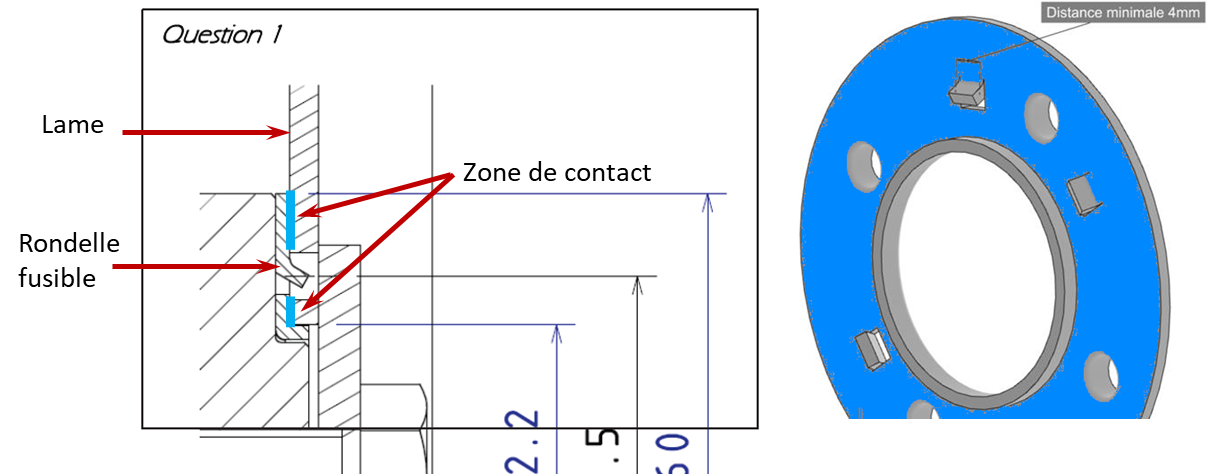
\includegraphics[width=14cm]{Q_01}
\end{center}

\end{UPSTIcorrige}

\UPSTIquestion Donner l'expression de $C_{{adh}}$ en fonction de $F_{{vis}}$, $\mu_{{acier/acier}}$, $D_{{int}}$ et $D_{{ext}}$.

\begin{UPSTIcorrige}
Le couple transmissible par adhérence lorsque la zone de contact est une seule couronne est donné par 
$C_{adh}=\frac{2}{3} \mu_{{acier/acier}}F_{{vis}} \frac{R^3-r^3}{R^2 - r^2}$.
 ou encore  $C_{adh}=\frac{2}{3} \mu_{{acier/acier}}F_{{vis}} \frac{2^2}{2^3}\frac{D_{{ext}}^3-D_{{int}}^3}{D_{{ext}}^2 - D_{{int}}^2}=\frac{1}{3} \mu_{{acier/acier}}F_{{vis}} \frac{D_{{ext}}^3-D_{{int}}^3}{D_{{ext}}^2 - D_{{int}}^2}$.
\end{UPSTIcorrige}


\UPSTIquestion Estimer la valeur de $C_{{adh}}$ (en \si{N.m}) à $\pm\SI{10}{\%}$.

\begin{UPSTIcorrige}
$C_{adh}=\frac{0,15}{3} \times 30000 \times \frac{60^3-32,2^3}{60^2 - 32,2^2}$
$\simeq 1500\times \frac{216000-27000}{3600 - 900}$
$\simeq 1500\times \frac{2000}{30}$
$\simeq 50\times 2000$
$\simeq \SI{100 000}{Nmm}$
soit $C_{adh}\simeq \SI{100}{Nm}$.

\textit{AN  -- Calculatrice : $C_{adh}\simeq \SI{107}{Nm}$.}

\end{UPSTIcorrige}

\subsection{Couple transmis par les ergots}

\UPSTIquestion* Sur le document réponse, cadre << question  4>>, identifier par un trait de couleur rouge la trace de la section cisaillée d'un ergot lors d'un choc sur la lame.

\begin{UPSTIcorrige}

\begin{center}
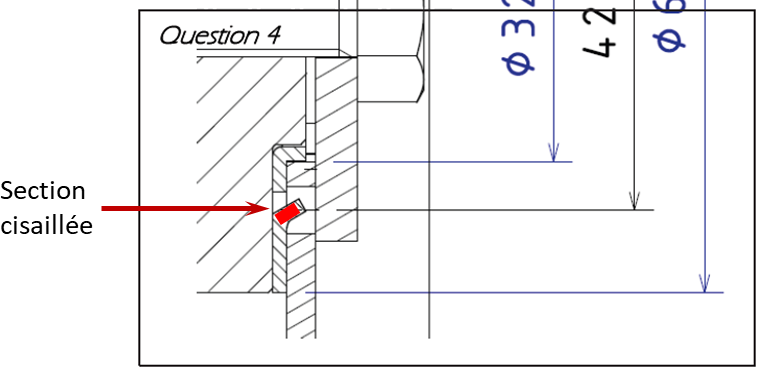
\includegraphics[width=10cm]{Q_04}
\end{center}
\end{UPSTIcorrige}

\UPSTIquestion Donner l'expression de $C_{cis}$ en fonction des données nécessaires. 

\begin{UPSTIcorrige}
La contrainte de cisaillement peut s'exprimer par $\sigma_c = \frac{F_c}{eb}$.
D'une part, il y a rupture de l'ergot lorsque $\sigma_c \geq R_m$. Au moment de la rupture, on fait donc l'hypothèse que
$R_m = \frac{F_c}{eb}$
D'autre part, pour un seul ergot, $C_{cis1} = F_c \frac{d_{ergot}}{2}$.
On a donc $C_{cis1} = R_m e b \frac{d_{ergot}}{2}$. 

Pour 4 ergots, $C_{cis} = 2R_m e b d_{ergot}$. 
\end{UPSTIcorrige}

\UPSTIquestion Estimer la valeur de $C_{cis}$ à  $\pm\SI{10}{\%}$.

\begin{UPSTIcorrige}
On a dans ce cas, $C_c = 2 \times 300 \times 1,5 \times  4 \times 42$
$ \simeq 2 \times 300 \times 252$ $ \simeq \SI{150000}{Nmm}$ $\simeq \SI{150}{Nm}$ .

\textit{AN -- Calculatrice : $C_{c}\simeq \SI{151}{Nm}$.}
\end{UPSTIcorrige}

\subsection{Couple transmis à l'arbre par la rondelle fusible lors d'un choix sur la lame}
\UPSTIquestion* Parmi les cinq expressions proposées dans le document réponse, cocher l'expression correcte de $C_{rond}$ en fonction de 
$C_{adh}$ et $C_{cis}$.

\begin{UPSTIcorrige}
Lors d'un choc, on veut que les ergots soient cisaillés. Pour cela il faut donc qu'il y ait glissement entre la rondelle et la lame puis que le couple généré par le choc cisaille les ergots. 
Nécessairement, on a donc $C_{rond}=C_{adh} + C_{cis}$.
\end{UPSTIcorrige}

\UPSTIquestion Donner la valeur de $C_{rond}$.

\begin{UPSTIcorrige}
En conséquence, $C_{rond} = MAX(120,200) = \SI{200}{Nm}$. 
\end{UPSTIcorrige}

\section{Détermination du couple transmis par le moteur électrique sur l'arbre au moment du démarrage}

\UPSTIquestion* Afin de déterminer $C_{mot}$, préciser l'ensemble isolé, cocher le principe retenu, le théorème utilisé et l'axe sur lequel il sera projeté (voir fig. 15, annexe B). 

\begin{UPSTIcorrige}
En utilisant l'hypothèse que l’intégralité du couple est transmise à l'arbre, on choisit d'isoler l'arbre de transmission, l'accouplement et la lame. 

Pour déterminer le couple moteur, on choisit << naturellement >> d'isoler l'arbre, d'appliquer le Principe Fondamental de la Dynamique et plus précisément le théorème du moment dynamique en $A$ en projection sur l'axe de rotation à savoir sur l'axe $\left(A,\overrightarrow{x_a}\right)$.
 \end{UPSTIcorrige}

\UPSTIquestion Donner l'expression de $C_{mot}$ en fonction des données de $J_{lame}$, $N_{arbre}$ et $\Delta t_{acc}$. 

\begin{UPSTIcorrige}
On isole l'arbre.

Bilan des actions mécaniques :
\begin{itemize}
\item action de la poulie sur l'arbre : $  C_{poulie\rightarrow arbre} = C_{mot}$ (en utilisant les hypothèses).
\end{itemize}

TMD sur l'axe $\left(A,\overrightarrow{x_a}\right)$ :
$  C_{mot} = \left(J_{lame}+J_{arbre}+J_{eq}\right) \dot{\omega}_{arbre}$.

Par ailleurs, $\omega_{arbre}  = N_{arbre} \frac{2\pi}{60}$ et  $\dot{\omega}_{arbre} = N_{arbre} \frac{2\pi}{60 \Delta t_{acc}}$.

Au final, $  C_{mot} = \left(J_{lame}+J_{arbre}+J_{eq}\right) N_{arbre} \frac{\pi}{30 \Delta t_{acc}}$.

Ne considérant que l'inertie de la lame, on a alors :$  C_{mot} = J_{lame} N_{arbre} \frac{\pi}{30 \Delta t_{acc}}$.
\end{UPSTIcorrige}

\UPSTIquestion Donner la référence de la lame (vour annexe C) qui est la plus exigeante pour dimensionner le couple moteur. 

\begin{UPSTIcorrige}
Au vu de l'expression précédente, la lame la plus exigeante est celle pour laquelle le produit 
$J_{lame} N_{arbre}$ est le plus grand. 

Pour la référence 37671 on a $J_{lame} N_{arbre} = 0,25 \times 2000 = \SI{500}{kg.m^2.tr.min^{-1}}$.

Pour la référence 42614 on a $J_{lame} N_{arbre} = 0,18 \times 3000 = \SI{540}{kg.m^2.tr.min^{-1}}$.

On choisit donc la référence 42614.
\end{UPSTIcorrige}


\UPSTIquestion Calculer le couple minimal $C_{mot\_min}$ que doit exercer le moteur sur l'arbre pour respecter $\Delta t _{acc}  = \SI{10}{s}$ quelle que soit la lame testée. 

\begin{UPSTIcorrige}
Dans les conditions précédentes, on aura donc 
:$  C_{mot\_min} = J_{lame} N_{arbre} \frac{\pi}{30 \Delta t_{acc}} =  \frac{540 \times \pi}{30 \times 10}$
$ \simeq \SI{5,4}{Nm}$ .

\end{UPSTIcorrige}


\section{Détermination du couple maximal transmissible par l'arbre}

\UPSTIquestion* Parmi les expressions proposées dans le document réponse, cocher l'expression correcte de $C_{arbre\_max}$ en fonction de $C_{rond}$ et $C_{mot\_max}$.
\begin{UPSTIcorrige}
Si le pieu est introduit à la fin de la phase d'accélération, il faut donc que l'arbre de transmission résiste à l'action conjointe du moteur et de la rondelle fusible. 

En conséquence, $C_{arbre_max} = C_{mot\_max}+ C_{rond}$.
\end{UPSTIcorrige}

\UPSTIquestion Donner la valeur de $C_{arbre\_max}$.

\begin{UPSTIcorrige}
$C_{arbre\_max} = 10+ 200 = \SI{210}{Nm}$.
\end{UPSTIcorrige}


\UPSTItitrePartieCorrige{Prédimensionnement de l'arbre}
\section{Étude de l'arbre en flexion exclusivement}

\UPSTIquestion* Exprimer les composantes des forces des paliers B et C sur l'arbre en fonction des données.

\begin{UPSTIcorrige}
On réalise le théorème de la résultante statique : 
\begin{itemize}
\item projection sur $\overrightarrow{x_a}$ : $B_x   = 0$;
\item projection sur $\overrightarrow{y_a}$ : $F_{lame/arbre} + B_y + C_y - F_{courroie/arbre}  = 0$. 
\end{itemize}
On réalise le théorème du moment statique en B: 
\begin{itemize}
\item projection sur $\overrightarrow{z_a}$ : $-F_{lame/arbre} \ell_1 + C_y \ell_2 - F_{courroie/arbre}\left(\ell_3 + \ell_2\right)=0$.
\end{itemize}

Résolution :
\begin{itemize}
\item $B_x   = 0$;
\item $ C_y = F_{courroie/arbre}\frac{\ell_3 + \ell_2}{\ell_2} + F_{lame/arbre} \frac{\ell_1}{\ell_2}$;
\item $B_y = F_{courroie/arbre} -  C_y -  F_{lame/arbre} = F_{courroie/arbre} -F_{courroie/arbre}\frac{\ell_3 + \ell_2}{\ell_2} - F_{lame/arbre} \frac{\ell_1}{\ell_2}-  F_{lame/arbre} $
$= F_{courroie/arbre}\left(1-\frac{\ell_3 + \ell_2}{\ell_2}\right) - F_{lame/arbre} \left(1+\frac{\ell_1}{\ell_2}\right) $
$= -F_{courroie/arbre}\frac{\ell_3}{\ell_2} - F_{lame/arbre} \left(1+\frac{\ell_1}{\ell_2}\right) $.
\end{itemize}

\end{UPSTIcorrige}

\UPSTIquestion Calculer les valeurs de composantes des forces des paliers B et C sur l'arbre.

\begin{UPSTIcorrige}
\begin{itemize}
\item $B_x   = 0$;
\item $C_y = 300 \frac{100 + 200}{200} + 1200 \frac{100}{200}$ $= 450 + 600 = \SI{1050}{N}$;
\item $B_y = -300\times \frac{100}{200} - 1200 \left(1+\frac{100}{200}\right) $ 
$=-\frac{1}{2}\times 300 - \frac{3}{2}\times 1200 = -150 - 1800 = -\SI{1950}{N} $ .
\end{itemize}\end{UPSTIcorrige}

\UPSTIquestion Donner l'expression des moments de flexion $M_{fzAB}(x_a)$ et $M_{fzBC}(x_a)$ en fonction des données $B_x$, $B_y$, $C_x$ ou $C_z$.

\begin{UPSTIcorrige}
\begin{itemize}
\item Pour $x_a \in [0,\ell_1]$, on isole $I$ : $\torseurstat{T}{II}{I} + \torseurstat{T}{lame}{arbre} = 0$.  On  a alors 
$M_{fz AB}(x_a) = x_a  F_{lame/arbre}$. 
\item Pour $x_a \in [\ell_1, \ell_1+\ell_2]$, on isole $I$ : $\torseurstat{T}{II}{I} + \torseurstat{T}{lame}{arbre} + \torseurstat{T}{0}{arbre} = 0$.
On  a alors $M_{fz BC}(x_a) = x_a  F_{lame/arbre} + \left(x_a - \ell_1\right) B_y$. 
\end{itemize}

\textbf{Non demandé}
\begin{itemize}
\item Pour $x_a \in [\ell_1+\ell_2,\ell_1+\ell_2+\ell_1]$, on isole $II$ : $\torseurstat{T}{I}{II} + \torseurstat{T}{courroie}{arbre} = 0$ soit $\torseurstat{T}{II}{I} =\torseurstat{T}{courroie}{arbre} $.  On  a alors 
$M_{fz AB}(x_a) = -  F_{courroie/arbre} (\ell_1+\ell_2+\ell_1-x_A)$. 
\end{itemize}

\end{UPSTIcorrige}

\UPSTIquestion Calculer les valeurs des moments de flexion en $B$ et $C$.

\begin{UPSTIcorrige}
\begin{itemize}
\item $M_{fz AB}(\ell_1) = \ell_1  F_{lame/arbre}$ $=\SI{30}{Nm}$.
\item $M_{fz BC}(\ell_1+\ell_2) =(\ell_1+\ell_2)  F_{lame/arbre} + \left(\ell_1+\ell_2 - \ell_1\right) B_y$
$=(\ell_1+\ell_2)  F_{lame/arbre}  +\ell_2 B_y$
$=300\times 1200+200 \times -1950$
$= 360 000-390 000$
$= -\SI{30}{Nm}$.
\end{itemize}

\end{UPSTIcorrige}

\UPSTIquestion Tracer l'évolution du moment de flexion $M_{fz}(x_a)$ dans l'arbre en précisant les caleurs significatives. 

\begin{UPSTIcorrige}
\begin{center}
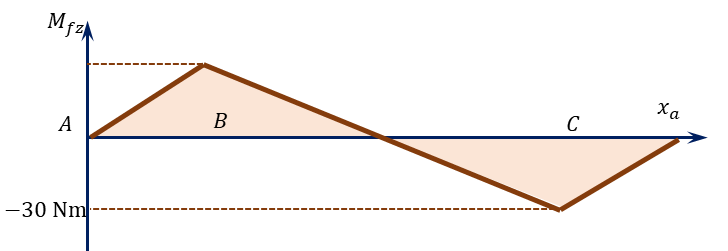
\includegraphics[width=10cm]{Q_19}
\end{center}
\end{UPSTIcorrige}

\UPSTIquestion Identifier le point où le moment de flexion est maximal et donner l'expression de $M_{fz-maxi}$.

\begin{UPSTIcorrige}
En $B$ et en $C$ la valeur du moment de flexion est identique, en valeur absolue. 

On a vu précédemment que $M_{fz AB}(\ell_1) = \ell_1  F_{lame/arbre}$ $=\SI{30}{Nm}$.
\end{UPSTIcorrige}

\UPSTIquestion Donner l'expression de la contrainte normale maximale dans une section droite $\sigma_{max\_sect}$ en fonction de $M_{fz}(x_a)$ et de $d_{flexion}$.

\begin{UPSTIcorrige}
La contrainte est donnée par $\sigma = -\frac{M_{fz}}{I_{Gz}}y$.

On a, pour une poutre cylindrique, $I_{Gz} = \frac{\pi d_{flexion}^4}{64} $. 

On a donc $\sigma_{max\_sect} = \frac{M_{fz}}{I_{Gz}} \frac{d_{flexion}}{2}$ 
$= \frac{M_{fz}}{\frac{\pi d_{flexion}^4}{64}} \frac{d_{flexion}}{2}$
$= \frac{32 M_{fz}}{\pi d_{flexion}^3} $.
\end{UPSTIcorrige}

\UPSTIquestion Exprimer le diamètre minimum de l'arbre de flexion $d_{flexion\_mini}$ en fonction de $s$, $R_e$ et des données identifiées précédemment. 

\begin{UPSTIcorrige}
En tenant compte du coefficient de sécurité, on souhaite nécessairement que 
$\sigma_{max\_sect} < \frac{Re}{s}$ soit $ \frac{32 M_{fz}}{\pi d_{flexion}^3}  < \frac{Re}{s}$.

Au final,  $d_{flexion}> \sqrt[3]{\frac{32 s M_{fz}}{Re \pi }} $.

\end{UPSTIcorrige}

\UPSTIquestion Calculer le diamètre minimum de l'arbre en flexion $d_{flexion\_mini}$. On pourra s'appuyer sur la figure 21 de l'annexe E. 

\begin{UPSTIcorrige}
Avec $ M_{fz} = \SI{30}{Nm}$, $d_{flexion}> \sqrt[3]{\frac{32 \times 2 \times 30 000}{300 \times \pi }} $ 
$ \Rightarrow d_{flexion}> \sqrt[3]{\frac{32 \times 2000 }{10 \times \pi }} $
$ \Rightarrow d_{flexion}> \sqrt[3]{2200} $ au final $d_{flexion}> \SI{13}{mm}$.

\end{UPSTIcorrige}


\section{Étude de l'arbre en torsion exclusivement}
\UPSTIquestion* En isolant l'ensemble \{arbre, poulie réceptrice\}, écrire le théorème du moment dynamique en projection sur l'axe $\overrightarrow{x_a}$.

\begin{UPSTIcorrige}
En reprenant un raisonnement précédent, 
$  C_{mot}+C_{rond\rightarrow arbre} = \left(J_{lame}+J_{arbre}+J_{eq}\right) \dot{\omega}(t)$
\end{UPSTIcorrige}

\UPSTIquestion En isolant uniquement l'arbre, écrire le théorème du moment dynamique en projection sur l'axe $\overrightarrow{x_a}$.

\begin{UPSTIcorrige}
Dans ce cas, on a 
$  C_{poulie \rightarrow arbre}+C_{rond\rightarrow arbre} = J_{arbre} \dot{\omega}(t)$
\end{UPSTIcorrige}

\UPSTIquestion En considérant que le moment d'inertie de l'arbre est négligeable devant les autres moments d'inertie, écrire la relation liant $C_{rond\rightarrow arbre}$ et $C_{poulie\rightarrow arbre}$.

\begin{UPSTIcorrige}
Dans ces conditions, on a donc $  C_{poulie \rightarrow arbre}+C_{rond\rightarrow arbre} =0$.
\end{UPSTIcorrige}

\section{Analyse des résultats}

\UPSTIquestion* Quelle proposition du document réponse retenez-vous pour déterminer le diamètre minimum de l'arbre ?

\begin{UPSTIcorrige}
Au vu des résultats précédents, on doit combiner les sollicitations de torsion et de flexion pour déterminer $dmini\_arbre$.
En effet la flexion produit des contraintes normales et la torsion produit des contraintes tangentielles, on ne 
connaît pas le critère de plasticité retenu.
\end{UPSTIcorrige}

\UPSTIquestion Les dimensions du châssis et de l'abre ne sont pas figés à ce stade de l'étude. Il est encore possible de faire évoluer les longueurs $l_1$, $l_2$ et $l_3$. A-t-on intérêt à les augmenter ou les diminuer ? Compléter le document réponse en justifiant les choix effectués. 

\begin{UPSTIcorrige}
%La sollicitation de torsion étant prépondérante, il n'ya aucun intérêt, du point de vue du dimensionnement de l'arbre, de modifier les longueurs $l_1$, $l_2$ et $l_3$.
La part de torsion est indépendante des longueurs, mais pas la flexion, il faut diminuer cette part en diminuant $l_1$ et $l_3$.
\end{UPSTIcorrige}


\UPSTItitrePartieCorrige{Étude du ressort d'éjection du pieu}
\section{Détermination de l'énergie nécessaire à l'éjection du pieu}

\UPSTIquestion* Donner l'expression de la masse du pieu en fonction de son diamètre $D_{pieu}$, de sa longueur $L_{pieu}$ et de la masse volumique de l'acier $\rho_{acier}$. Précisez l'unité. 

\begin{UPSTIcorrige}
On a  $m_{pieu} = \rho_{acier} \frac{\pi D^2_{pieu}}{4} L_{pieu}$ avec $\rho_{acier}$ en $\si{kg.m^{-3}}$. 
\end{UPSTIcorrige}

\UPSTIquestion Donner une valeur numérique pour la masse volumique (deux chiffres significatifs) d'un acier standard $\rho_{acier}$. Précisez l'unité. 

\begin{UPSTIcorrige}
Pour un acier standard, la masse volumique est comprise entre \SI{7200}{kg.m^{-3}} et \SI{7800}{kg.m^{-3}}.
\end{UPSTIcorrige}

\UPSTIquestion Calculer la masse du pieu $m_{pieu}$. Précisez l'unité. 

\begin{UPSTIcorrige}
$m_{pieu} = 8000 \times \frac{3\times 25^2}{4} \times 360 \times 10^{-9}$
$= 8000 \times 625\times 270 \times 10^{-9}$
$\simeq 8 \times625\times 27 \times 10^{-5}$
$\simeq 5\times 27 \times 10^{-2}$
$\simeq \SI{1,5}{kg}$.


\end{UPSTIcorrige}


\UPSTIquestion Compte tenu des indications précédentes, donner la valeur numérique de la course $\Delta L_{finale}$. 

\begin{UPSTIcorrige}

%\textbf{*** A confirmer} 
La seule indication utilisable semble le figure 22 annexe F selon laquelle  $\Delta L_{finale} = 20 + 4 = \SI{24}{mm}$.

\end{UPSTIcorrige}

\UPSTIquestion Écrire la relation littérale puis calculer $t_{\Delta finale}$, en secondes.
\begin{UPSTIcorrige}
Le pieu peut avancer lors de l'absence de la lame, c'est à dire pendant que la lame se déplace de \SI{105}{\degres}. 
À une vitesse de $\SI{3500}{tr.min^{-1}} = 3500\times \frac{360}{60} \si{\degres.s^{-1}} =   \SI{21000}{\degres.s^{-1}}$. Pour parcourir \SI{105}{\degres} à cette vitesse, il faut $\frac{105}{21000} \simeq \frac{100}{20000} \simeq \SI{5}{ms}$. 

Au final, $t_{\Delta finale} = \SI{5}{ms} $
\end{UPSTIcorrige}

\UPSTIquestion Écrire la relation littérale puis calculer la vitesse du pieu $V_{finale}$, en $\si{m.s^{-1}}$.

\begin{UPSTIcorrige}
En faisant l'hypothèse que le pieu se déplace à vitesse constante, on a $V_{finale} = \frac{\Delta L_{finale}}{t_{\Delta finale}}$.

On a donc $V_{finale} = \frac{24}{5 \times 10 ^{-3}}  = \SI{4,8}{m.s^{-1}}$. 


\end{UPSTIcorrige}

\UPSTIquestion Écrire la relation littérale puis calculer l'énergie cinétique du pieu $E_{finale tir}$. 

\begin{UPSTIcorrige}
Pour un solide en translation, l'énergie cinétique est donnée par : $E_{finale tir} = \frac{1}{2}m_{pieu} V_{finale}^2$.

On a donc $E_{finale tir} = \frac{1}{2} \times 1,5 \times 4,8^2 \simeq 0,75 \times 25 = \SI{18,75}{J}$.

%\textit{AN : $E_{finale tir} = \SI{1728}{J}$.}
\end{UPSTIcorrige}

\section{Dimensionnement du ressort propulseur}
\subsection*{Choix n°1}

\UPSTIquestion* Sur la figure 23 de l'annexe G, que représente l'aire grisée ?
En déduire la course du tir $C_{poussée choix 1}$ correspondant à ce choix 1. Écrire la relation littérale puis effectuer le calcul numérique. 

\begin{UPSTIcorrige}
Il s'agit de la zone dans laquelle on peut armer le ressort, sans dépasser l'effort acceptable que peut fournir l'opérateur. 

%On a $F_{op acc choix 1} = KC_{poussée choix 1}$ et donc $C_{poussée choix 1} = \frac{K}{F_{op acc choix 1}}$.
%
%Au final, $C_{poussée choix 1} = \frac{K}{F_{op acc choix 1}}$. On ne connait pas $K$.

L'aire grisée représente le travail de l'opérateur pour comprimer le ressort. 
On note $W = \frac{1}{2} F_{op acc choix 1}C_{poussée choix 1}$ ce travail. 
Par ailleurs, on a $E_{ressort} = \SI{20}{J}$ l'énergie que doit restituer le ressort. 

En conséquence,  $C_{poussée choix 1} = \frac{2 E_{ressort}}{F_{op acc choix 1}}$ 
soit $C_{poussée choix 1} =\frac{2\times 20}{190}\simeq \frac{2\times 20}{200}\simeq \SI{0,2}{m}$.

\end{UPSTIcorrige}


\subsection*{Choix n°2}
\UPSTIquestion* Sur le document réponse, compléter la figure en ajoutant les éléments suivants : 
\begin{itemize}
\item évolution de la force développée par le ressort;
\item $F_{fin\, poussee\, choix 2}$;
\item le travail du ressort pendant la poussée.
\end{itemize}

\begin{UPSTIcorrige}
\begin{center}
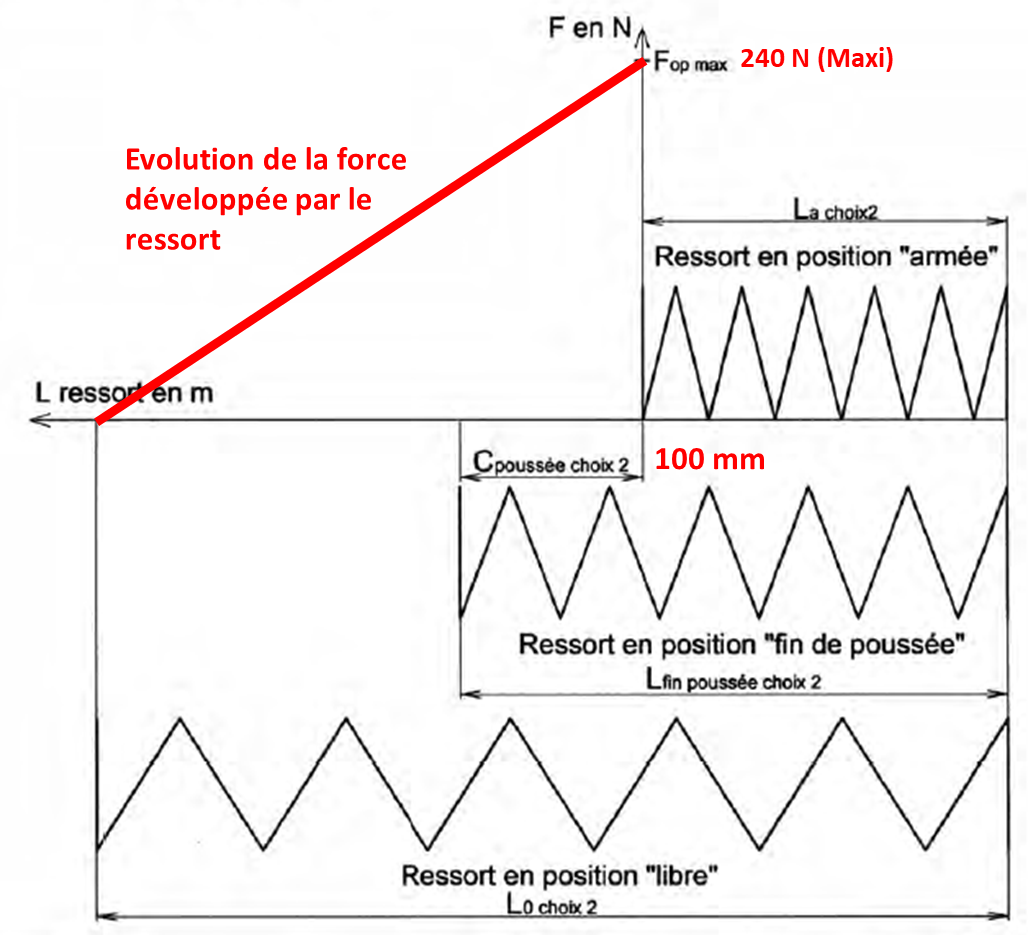
\includegraphics[width=10cm]{Q_37}
\end{center}
Le travail du ressort correspond à l'aire du trapèze.
\end{UPSTIcorrige}

\UPSTIquestion De la figure précédente, déduire l'expression littérale de $F_{fin pouss\'ee choix 2}$ en fonction de $E_{ressort}$, $F_{op max choix 2}$ et $C_{pouss\'ee choix 2}$ puis effectuer le calcul numérique. 

\begin{UPSTIcorrige}
L'énergie à restituer correspond dès lors à l'aire du trapèze. On a donc 

$E_{ressort} = \frac{1}{2}\left(F_{op max choix 2} + F_{fin pouss\'ee choix 2} \right)C_{pouss\'ee choix 2}$. 

On a alors $ F_{fin pouss\'ee choix 2} = \frac{2 E_{ressort}}{C_{pouss\'ee choix 2}} - F_{op max choix 2}$.

AN : $ F_{fin pouss\'ee choix 2} = \frac{2 \times 20}{100\times 10^{-3}} - 240 =\SI{160}{N} $
\end{UPSTIcorrige}



\subsection*{Utilisation d'un configurateur en ligne}

\UPSTIquestion* En tenant compte des données et des résultats de vos calculs (choix 2), sur le document réponse, compléter uniquement les cases nécessaires de la fiche de calcul du constructeur.

\begin{UPSTIcorrige}
Valeurs à saisir : 
\begin{itemize}
\item $D_e = \SI{50}{mm}$;
\item $L_2 = \SI{100}{mm}$;
\item $F_2 = \SI{240}{N}$.
	\end{itemize}
\end{UPSTIcorrige}

\UPSTIquestion Donner l'expression puis calculer les efforts $F_{armée}$ du ressort proposé en position << armé >> et l'effort $F_{fin de tir}$ en position << fin de tir >>. 

Donner le diamètre extérieur nominal $D_{ext nominal}$ et calculer le diamètre extérieur $D_{ext max}$. Conclure. 

\begin{UPSTIcorrige}
Le ressort a une raideur de \SI{0,8}{N/mm}. La longueur à vide est de \SI{400}{mm}. La longueur armée est de \SI{100}{mm}. On a donc $F_{armée} = 300 \times 0,8 = \SI{240}{N}$. 

La course étant de $\SI{100}{mm}$, en fin de tir, on a donc $F_{fin de tir}= 200 \times 0,8 = \SI{160}{N}$

On lit sur l'annexe  $D_{ext nominal} = \SI{44,5}{mm}$. Ce qui est inférieur aux \SI{50}{mm} requis.

\end{UPSTIcorrige}

\subsection*{Identification des zones de contact}
\UPSTIquestion* Sur le document réponse, compléter la cotation de la bague << glycodur >> et du pêne. Calculer le jeu $J_{max}$ en mm.
\begin{UPSTIcorrige}


\begin{center}
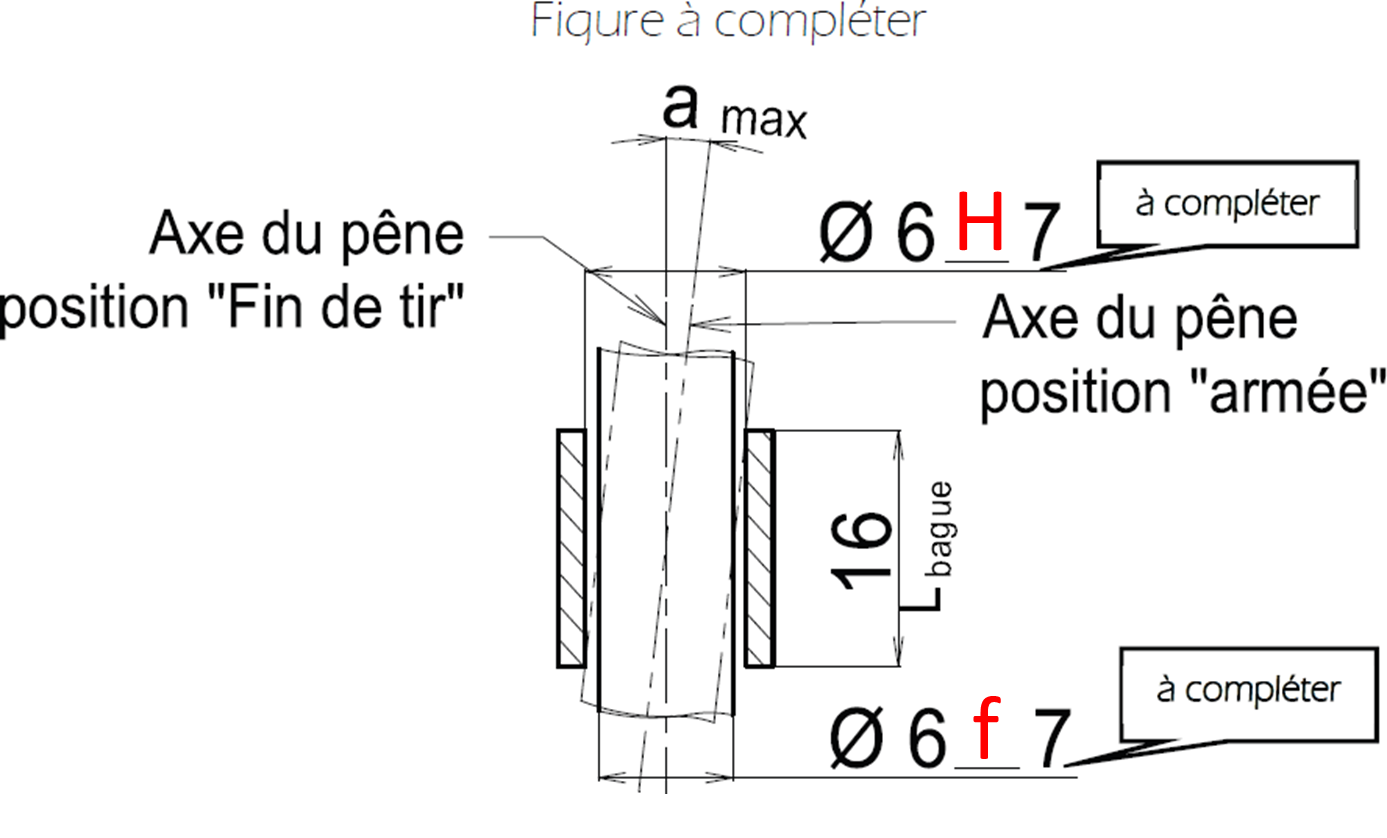
\includegraphics[width=14cm]{Q_41}
\end{center}

Le jeu est maximum pour le moyen le plus grand (\SI{6,012}{mm}) et l'arbre le plus petit (\SI{5,978}{mm}). Le jeu maximal est donc de \SI{0,034}{mm}.

\end{UPSTIcorrige}

\UPSTIquestion Exprimer de façon littérale puis estimer en radian la valeur de l'angle de rotulage $\alpha_{max}$.
Préciez l'hypothèse utilisée pour réaliser votre estimation d'angle. 
\begin{UPSTIcorrige}

\begin{center}
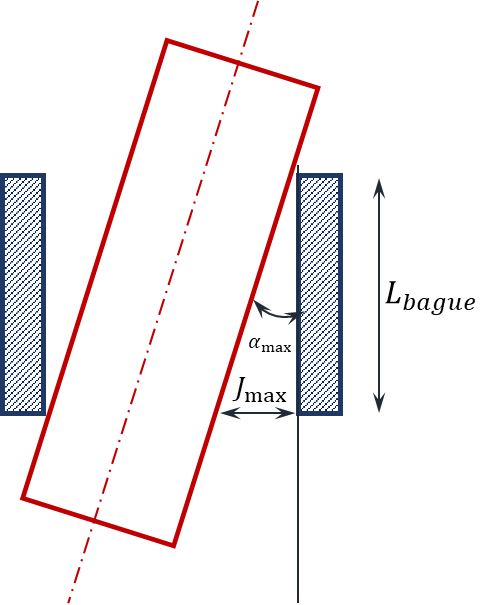
\includegraphics[width=6cm]{Q_42}
\end{center}

Lorsque le pêne rotule, on peut donc exprimer l'angle de rotulage par $\tan \alpha_{\text{max}} = \frac{J_{\text{max}}}{L_{\text{bague}}}$.

En faisant l'hypothèse que l'angle est petit, 
$\tan \alpha_{\text{max}} \simeq \alpha_{\text{max}} \simeq  \frac{0,034}{16}\simeq  \frac{32}{16} \times 10^{-3}\simeq  \SI{2e-3}{rad}$.
\end{UPSTIcorrige}

\subsection*{Détermination de l'effort à fournir par l'actionneur électromagnétique.}
\UPSTIquestion* Sur le document réponse, en position << tir >>, à l'échelle : 
\begin{itemize}
\item en rouge, tracer $P_N$, $Q_N$ et $R_N$;
\item en bleu, tracer $P_T$, $Q_T$ et $R_T$;
\item en bleu, tracer $\overrightarrow{F_{sol tir}}$.
\end{itemize}
Donner la valeur numérique de $P_T$, $Q_T$ et $R_T$.

\begin{UPSTIcorrige}
\begin{center}
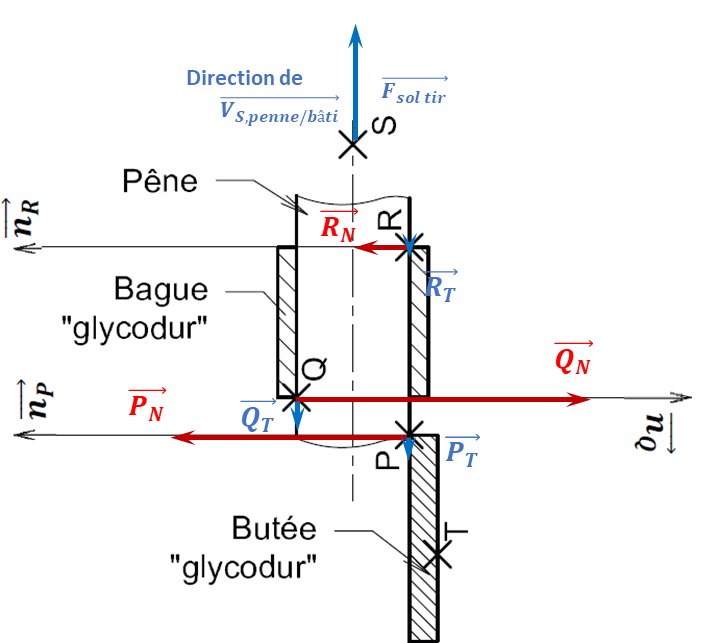
\includegraphics[width=12cm]{Q_43}
\end{center}

En utilisant les lois de Coulomb à la limite du glissement, on a $P_T=\SI{12}{N}$, $Q_T=\SI{15}{N}$ et $R_T=\SI{3}{N}$.
\end{UPSTIcorrige}

\UPSTIquestion Écrire l'expression littérale de la norme de $\overrightarrow{F_{sol tir}}$ et donner sa valeur numérique.
\begin{UPSTIcorrige}

$\overrightarrow{F_{sol tir}}$ s'obtient en isolant le pêne et en réalisant un théorème de la résultante statique en projection  sur l'axe vertical. On a donc $F_{sol tir} = P_T + Q_T + R_T = 12+15+3 = \SI{30}{N}$.

\end{UPSTIcorrige}

\UPSTIquestion Sur le document réponse, cocher la case correspondant au taux d'utilisation des actionneurs électromagnétiques du banc d'essai.

\begin{UPSTIcorrige}
%\textbf{Interprétation incertaine} : je pense que
Pour faire rentrer le pêne et libérer le poussoir, le temps d'alimentation du solénoïde doit être très faible. J'aurais tendance à dire que l'alimentation doit être de courte durée. 
\end{UPSTIcorrige}

\UPSTIquestion Parmi les trois actionneurs proposés, choisir celui ou ceux qui conviennent en entourant sur chaque graphique la zone de la courbe qui justifie ce choix.

\begin{UPSTIcorrige}
Les \SI{40}{N} doivent être maintenus pendant 8 mm de de course, afin que le pêne ne soit plus en contact avec le poussoir. Ainsi la courbe doit être compris dans le carré rouge afin de pouvoir maintenir un effort pendant une distance suffisamment grande. 

On opte pour le ER 40/C.

\begin{center}
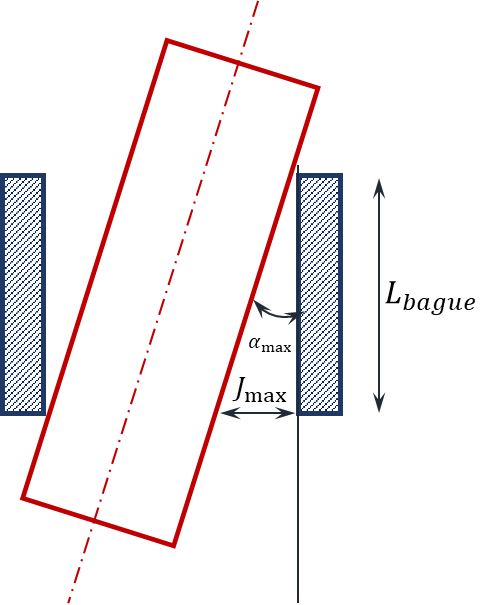
\includegraphics[width=6cm]{Q_42}
\end{center}


\end{UPSTIcorrige}


\UPSTItitrePartieCorrige{Dessin d'étude de Construction Mécanique}

\section{Platine de fixation 16}

\UPSTIquestion* Sur le document pré imprimé format A3, cadre << Mise en situation >> à l'échelle 1/2, choisir l'orientation du profilé donnant la meilleure rigidité du châssis en cochant la case S1 ou S2. 
\begin{UPSTIcorrige}
\end{UPSTIcorrige}

\UPSTIquestion Représenter votre proposition de solution pour la liaison complète entre la platine de fixation 16 et le bâti. Le maintien en position est déjà défini (6 vis et 6 écrous spéciaux pour profilé). Lorsque les vis ne sont pas serrées, le réglage de la position du canon par rapport au bâti doit être possible.
 
Indiquer la valeur des ajustements normalisés nécessaires.
\begin{UPSTIcorrige}
\end{UPSTIcorrige}

\UPSTIquestion Représenter votre proposition de solution pour la liaison complète (appui-plan + centrage court) démontable entre le fût 17 et la platine de fixation 16. 

Indiquer la valeur des ajustements normalisés nécessaires.
\begin{UPSTIcorrige}
\end{UPSTIcorrige}

\UPSTIquestion Représenter votre proposition de solution pour la liaison complète (appui-plan + centrage court) démontable entre le corps du propulseur 1 et la platine de fixation 16. Indiquer la valeur des ajustements normalisés nécessaires.

Cette liaison doit permettre également la mise et le maintien en position de la bague d'amortissement 15 entre la platine de fixation 16 et le corps du propulseur 1. 

\begin{UPSTIcorrige}
\end{UPSTIcorrige}

\section{Gâchette}

\UPSTIquestion* Représenter votre proposition de solution pour la liaison entre le pêne 10 et l'axe du solénoïde 13. Cette liaison ne doit permettre que la transmission de l'effort de déverrouillage. 

Les jeux permettant les degrés de liberté nécessaires au bon fonctionnement doivent être représentés (1mm minimum). 
\begin{UPSTIcorrige}
\end{UPSTIcorrige}

\UPSTIquestion Représenter votre proposition de solution pour la forme extérieure du poussoir 7 ainsi que la forme de l'extrémité du pêne 10, permettant, lors de l'aménagement, de repousser l'axe du solénoïde pour réaliser le verrouillage automatique du système. En position << armée >>, le contact linéique entre le pêne 10 et la bague << Glycodur >> 8 doit être de 2 mm au minimum.
\begin{UPSTIcorrige}
\end{UPSTIcorrige}

\section{Culasse 2 et poussoir 7}

\UPSTIquestion* La liaison complète entre la culasse 2 et le corps du propulseur 1 est partiellement réalisée. Le maintien en position par 3 vis est déjà défini. Représenter votre proposition de solution permettant la mise en position de la culasse 2 sur le corps du propulseur 1. 
\begin{UPSTIcorrige}
\end{UPSTIcorrige}

\UPSTIquestion Définir les formes de la culasse 2 permettant de guider le ressort propulseur3.
\begin{UPSTIcorrige}
\end{UPSTIcorrige}

\UPSTIquestion Représenter votre proposition de solution permettant la mise et le maintien en position des douilles à billes dans la culasse 2. 
\begin{UPSTIcorrige}
\end{UPSTIcorrige}

\UPSTIquestion Définir les formes du poussoir 7 permettant de guider le ressort propulseur 3.

 Représenter votre proposition de solution pour la liaison complète démontable entre le poussoir 7 et la tige d'armement 5. 
\begin{UPSTIcorrige}
\end{UPSTIcorrige}


\begin{center}
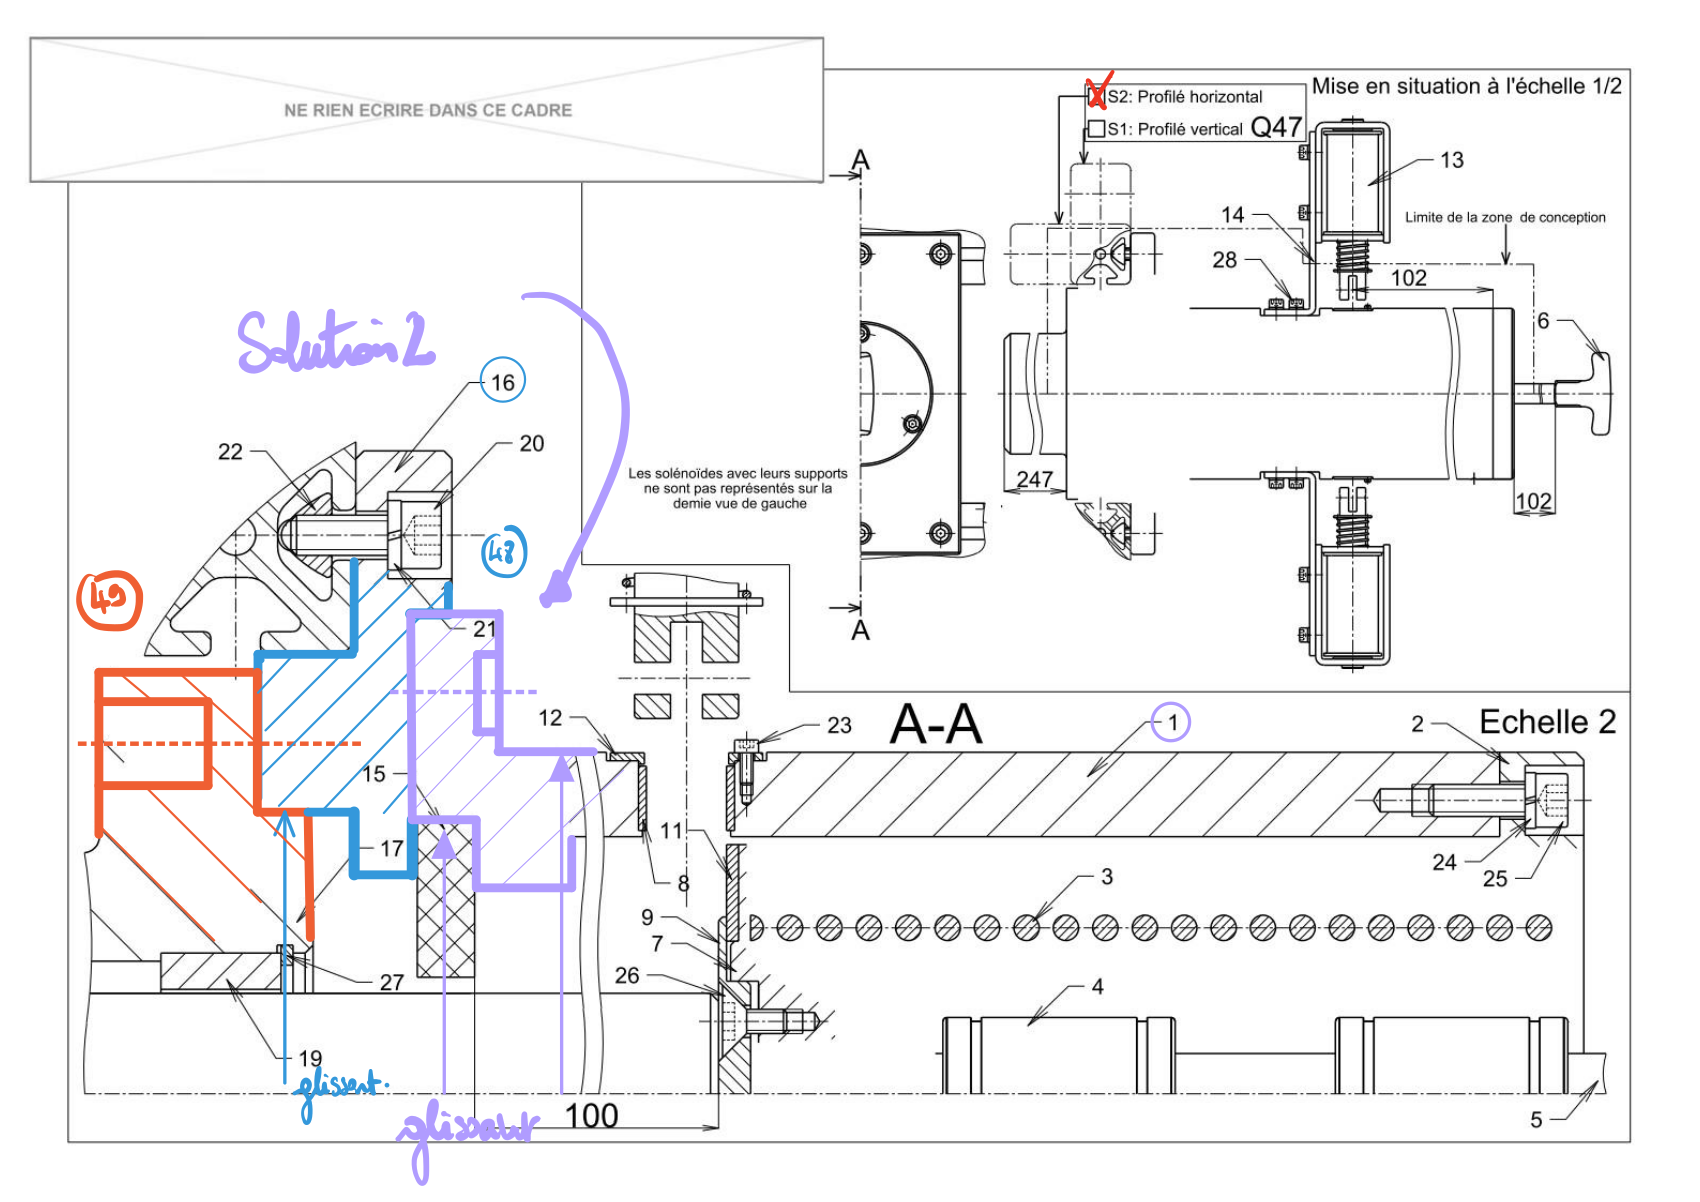
\includegraphics[width=\linewidth]{calque_01}
\end{center}

\begin{center}
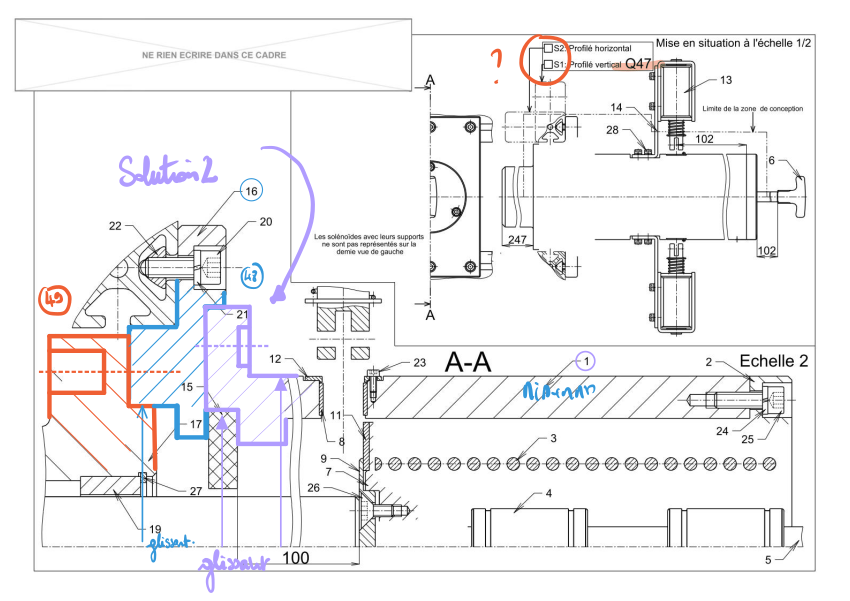
\includegraphics[width=\linewidth]{calque_02}
\end{center}

%\begin{center}
%\includegraphics[width=\linewidth,page=1]{croquis}
%\end{center}
%
%\begin{center}
%\includegraphics[width=\linewidth,page=2]{croquis}
%\end{center}

% -------------------------- 
% Boite d'objectif 
% -------------------------- 
%\UPSTIobjectif{
%Exemple d'objectif de partie...
%}
% -------------------------- 


\end{document}
